Now we have to configure the \texttt{nginx} server in order to expose our .NET Core web application to the outside.
As a result of this section web app will be exposed and accessible via VM's external IP address.
Let's install it using the commands
\begin{itemize}
    \item \texttt{sudo apt update -y}
    \item \texttt{sudo apt install -y nginx build-essential}
\end{itemize}
Terminal output:
\begin{figure}[H]
    \centering
    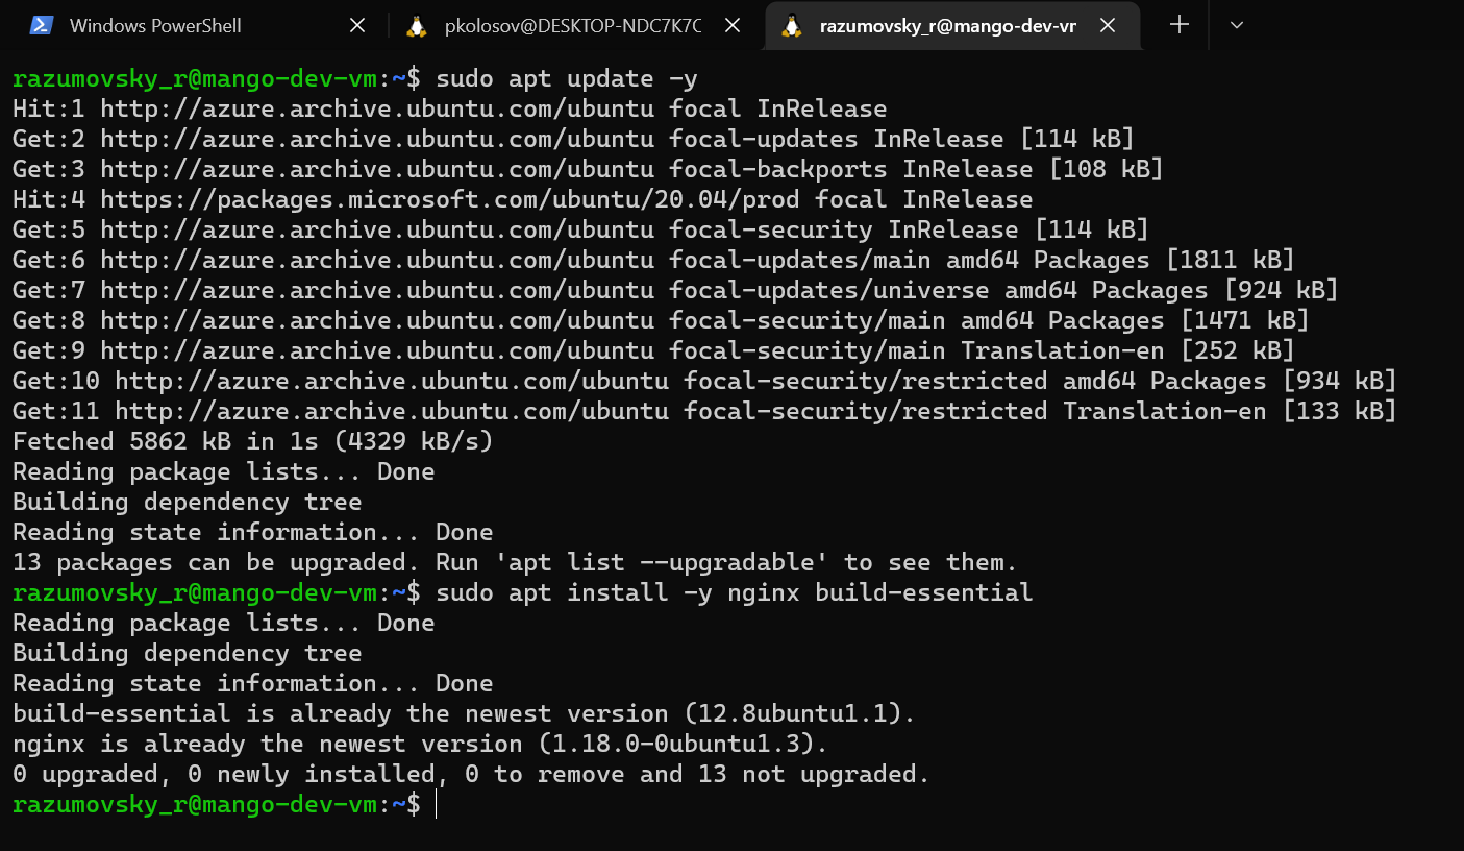
\includegraphics[width=1\textwidth]{img/06_install_nginx}
    ~\caption{Ubuntu install nginx terminal output.}\label{fig:figure15}
\end{figure}
Next, it is necessary to create nginx configuration~\cite{NginxConfig} that exposes our application, that is
\begin{spverbatim}
    server {
        server_name STATIC_IP_ADDRESS_OF_VM;

        location / {
            include proxy_params;
            proxy_pass http://127.0.0.1:8080;
        }

        location /swagger {
            include proxy_params;
            proxy_pass http://127.0.0.1:8080;
        }

        location /api {
            include proxy_params;
            proxy_pass http://127.0.0.1:8080;
        }

        location /notify {
            proxy_pass http://127.0.0.1:8080;
            proxy_http_version 1.1;
            proxy_set_header Upgrade $http_upgrade;
            proxy_set_header Connection "upgrade";
            proxy_set_header Host $host;
            proxy_cache_bypass $http_upgrade;
        }
    }
\end{spverbatim}
We create it at the following path on behalf of our Azure VM via SSH
\begin{center}
    \texttt{sudo vim /etc/nginx/conf.d/back.mangomesenger.company.conf}
\end{center}
Restart nginx and validate its state using the commands
\begin{itemize}
    \item \texttt{sudo systemctl restart nginx}
    \item \texttt{sudo nginx -t}
\end{itemize}
Terminal output:
\begin{figure}[H]
    \centering
    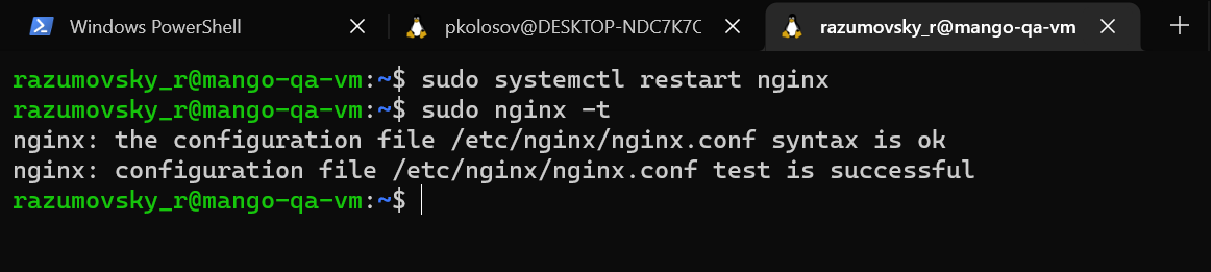
\includegraphics[width=1\textwidth]{img/06_test_nginx}
    ~\caption{Restart and test nginx terminal output.}\label{fig:figure16}
\end{figure}
Now we must be able to find our application listening to the
\begin{center}
    \texttt{http://STATIC\_IP\_ADDRESS\_OF\_THE\_VM}
\end{center}
And actually it works as expected
\begin{figure}[H]
    \centering
    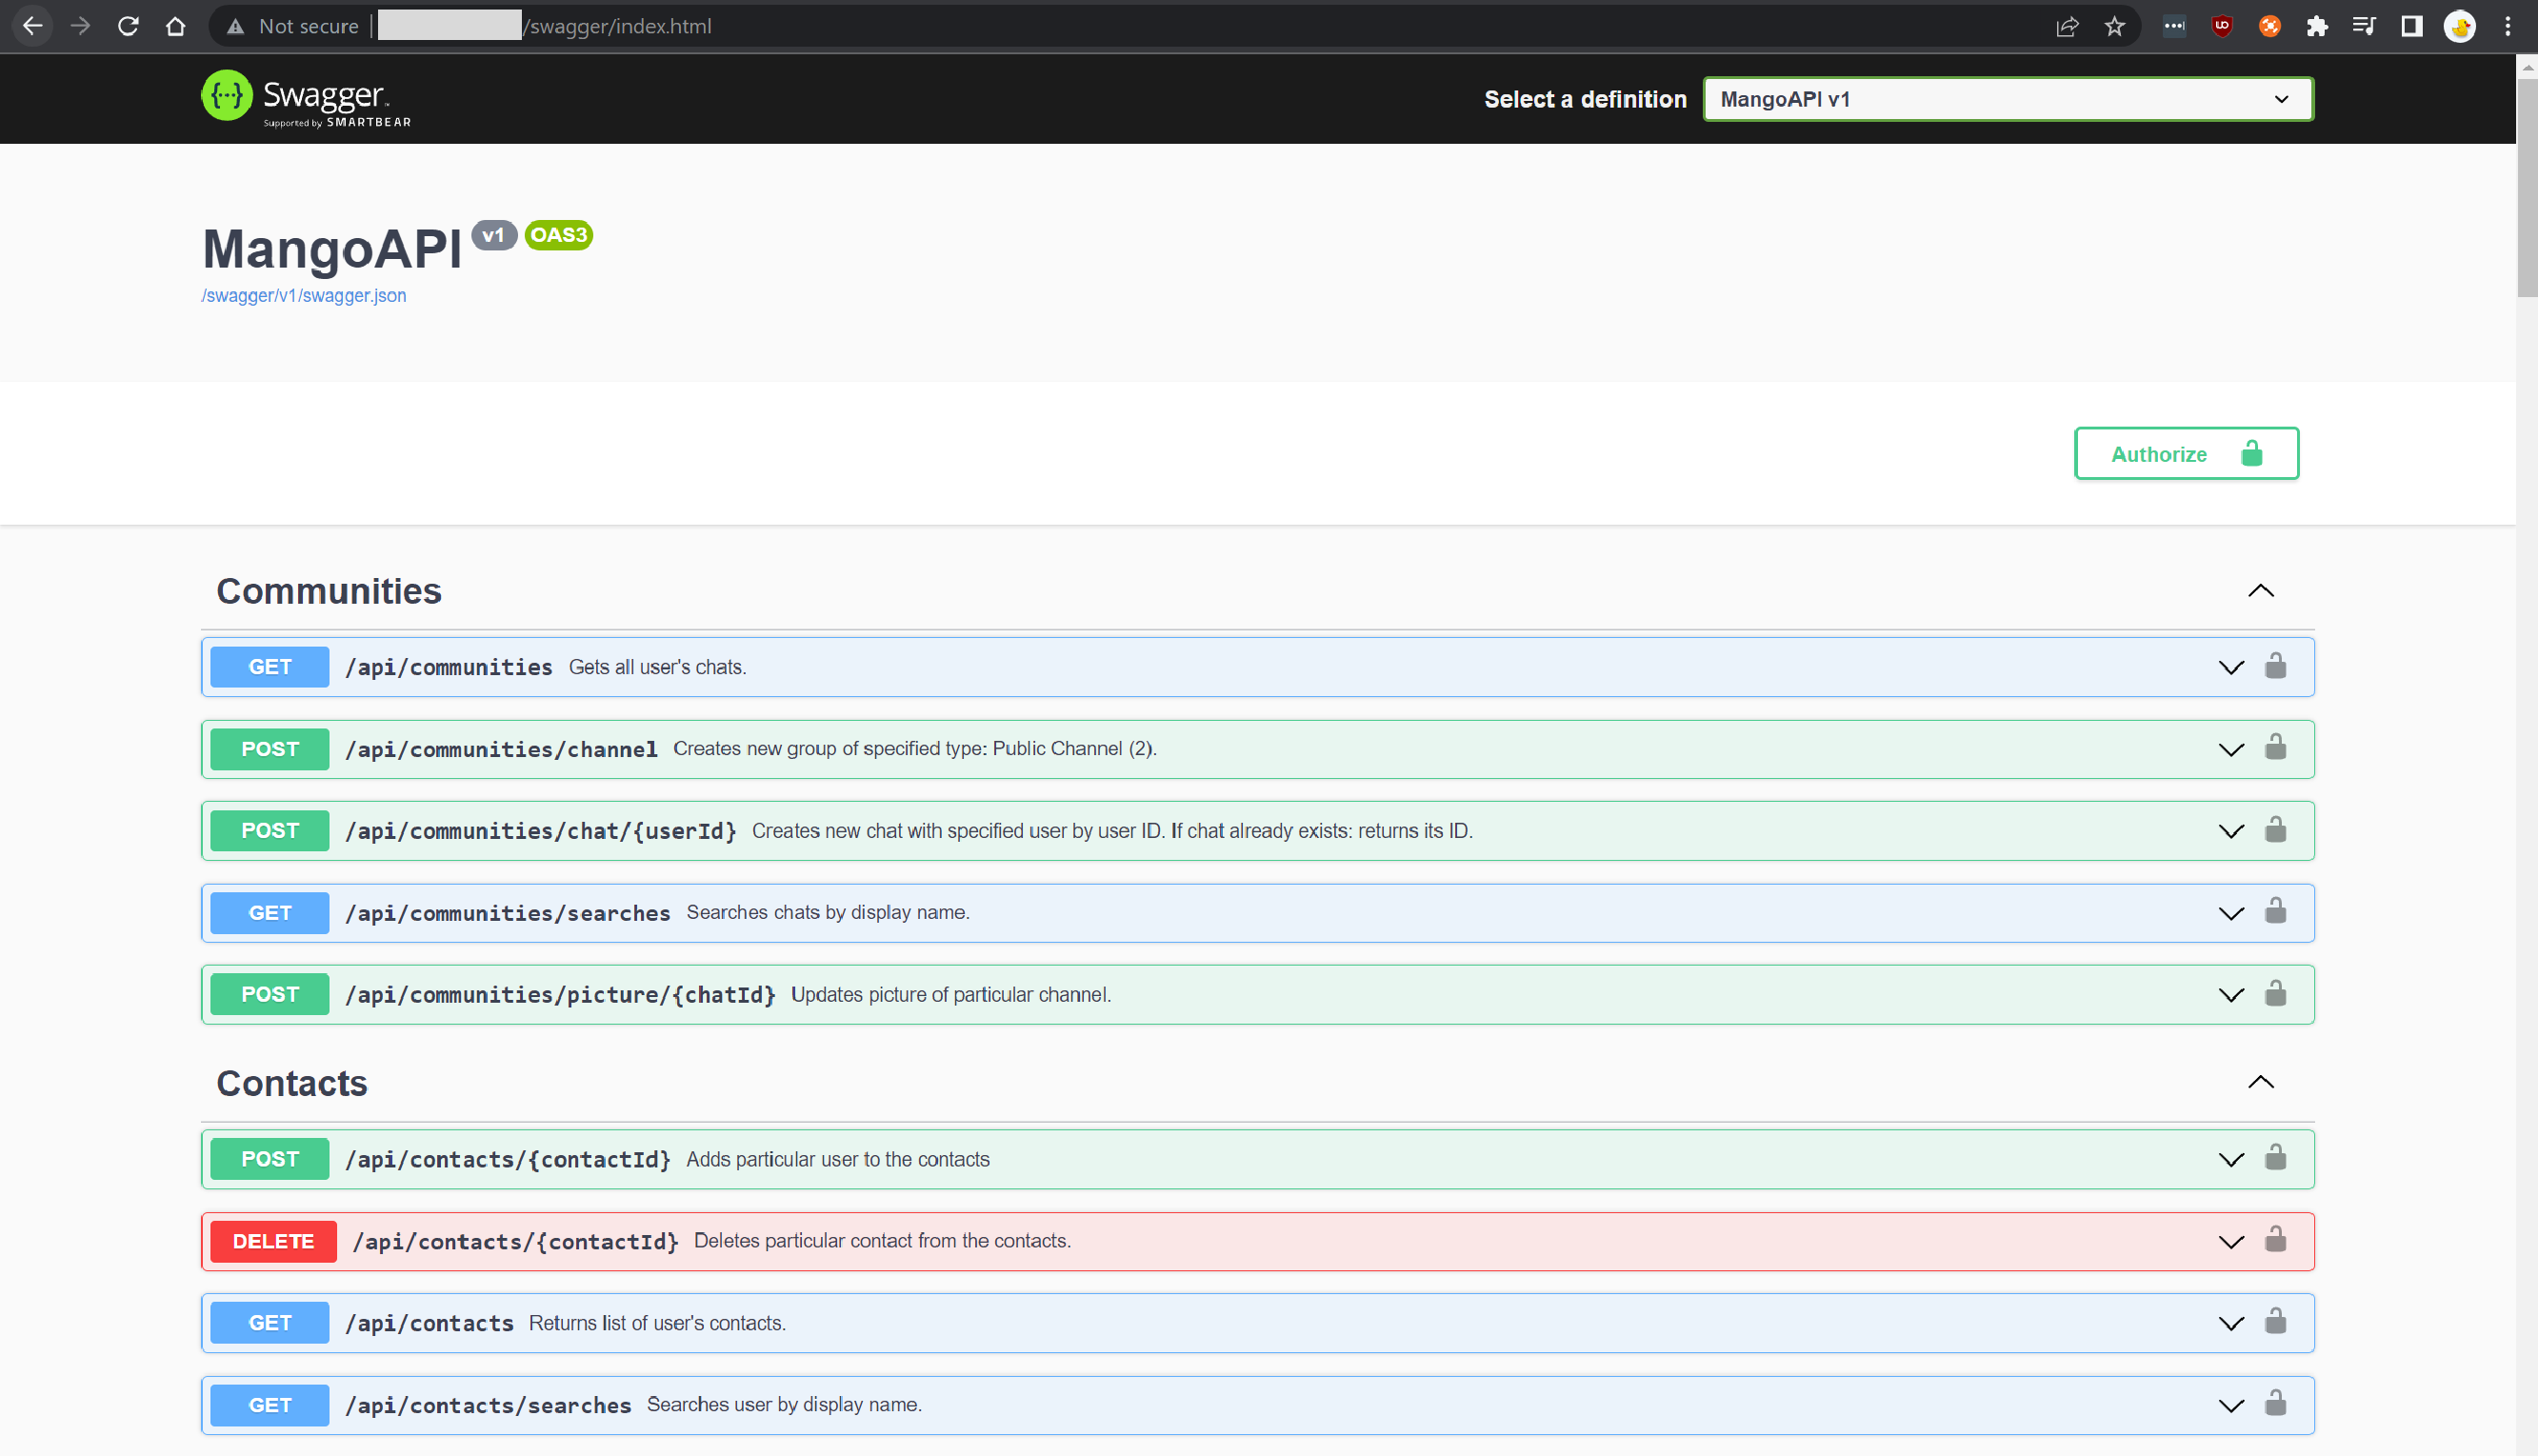
\includegraphics[width=1\textwidth]{img/06_view_in_browser}
    ~\caption{.NET Core web app accessed via browser using static IP address of the virtual machine.}\label{fig:figure17}
\end{figure}
In this section we have installed and configured the \texttt{nginx} web server so that it exposes our .NET Core web
application (run on behalf of Ubuntu service) from the previous section and makes it available
from the web browser under the url \texttt{http://STATIC\_IP\_ADDRESS\_OF\_THE\_VM}.